\section*{Question 7}

\paragraph{(a)} We extend the model by adding the recession state $r_t \in \{0,1\}$ as a state variable. The aggregate shock function becomes $\lambda(y_t, r_t) = \lambda_0 + \lambda_1 r_t$, so equation (6) is modified to
\[
  w_t = \exp(\alpha_b + \gamma k_t)\cdot(1 + \lambda_0 y_t + \lambda_1 r_t). \tag{6$'$}
\]
All other equations (1)--(5), (7)--(11) are unchanged. The state space expands from $(b, k_t)$ to $(b, k_t, r_t)$, and the Bellman equation (11) is now
\[
  V(t,b,k,r) = \max_{l \in [0,1]} \left\{ U(c,l) + \beta \sum_{r' \in \{0,1\}} \Pr(r_{t+1}=r'\mid r_t=r)\sum_{\varepsilon} p_\varepsilon \, V(t+1,b,k',r') \right\},
\]
where $k' = \bigl((1-\delta)k + l\bigr)\varepsilon$, $c$ is given by (3), and transition probabilities follow Table~1. The solution requires solving for $V$ and $l^*$ over the expanded grid $(t, b, k, r)$, integrating simultaneously over both the recession transition and the human capital shock.

\paragraph{(b)} We solve and simulate the model with $\lambda_1 = -0.5$. The recession path $\{r_y\}$ from Figure~1 is applied identically to all workers in year $y$:
\[
  r_y = [0,0,0,1,1,0,0,0,0,1,1,0,0,0,0,0,0,1,0,0,0,0,1,1], \quad y=1,\ldots,24.
\]

\paragraph{(c)} Figure~\ref{fig:q7_age} shows average labor supply, consumption, and recession exposure as a function of age. Each age cell pools all birth cohorts present at that age, so the recession frequency in panel~(c) reflects the overlap between cohort life cycles and the exogenous recession path.

\begin{figure}[H]
  \centering
  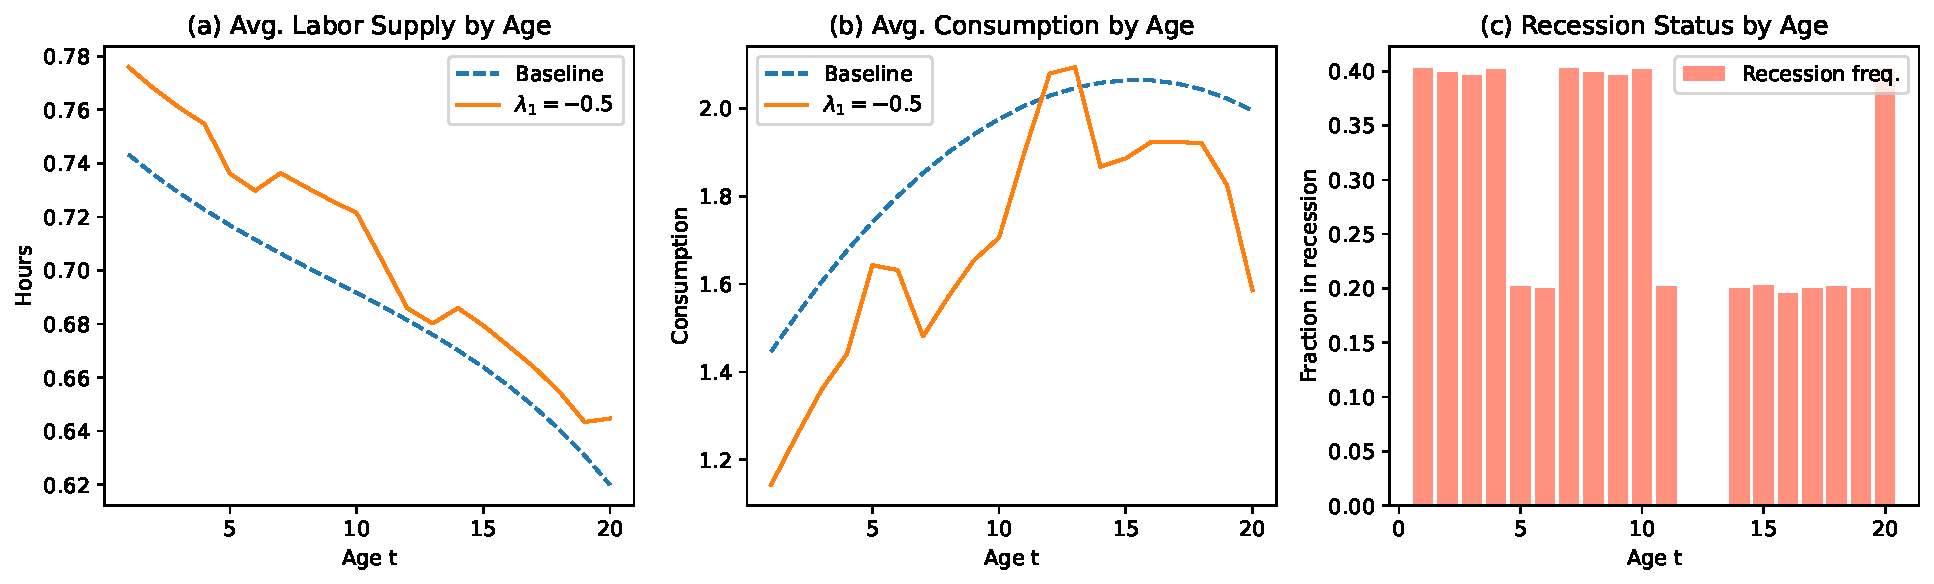
\includegraphics[width=\textwidth]{../figures/q7_age_profiles.pdf}
  \caption{Age profiles under $\lambda_1 = -0.5$ (solid) vs.\ baseline $\lambda_1 = 0$ (dashed). Panel (c): fraction of workers experiencing a recession year at each age.}
  \label{fig:q7_age}
\end{figure}

\paragraph{(d)} Figure~\ref{fig:q7_year} shows the same variables by calendar year. Because all workers in year $y$ share the same $r_y$, the recession indicator in panel~(c) is simply the exogenous path from Figure~1. The labor supply and consumption series track it sharply but in \emph{opposite} directions: in each recession year average labor supply jumps \emph{up} (by about $+0.065$) while consumption drops steeply (by $0.7$--$1.1$), with both reverting in the following non-recession year.

\begin{figure}[H]
  \centering
  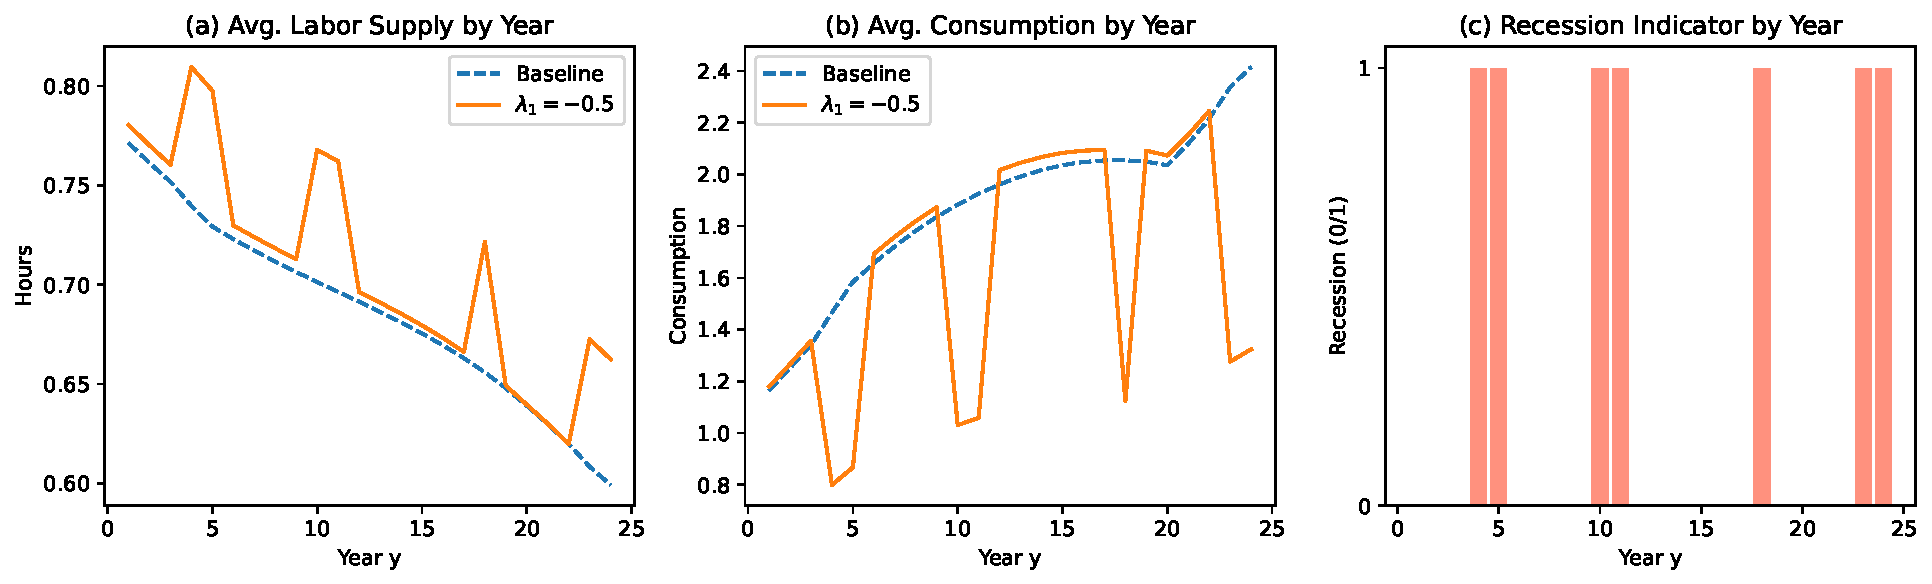
\includegraphics[width=\textwidth]{../figures/q7_year_profiles.pdf}
  \caption{Year profiles under $\lambda_1 = -0.5$ (solid) vs.\ baseline (dashed). Bars in panel (c) mark recession years ($r_y = 1$).}
  \label{fig:q7_year}
\end{figure}

\paragraph{(e)} A recession scales all wages down by $\lvert\lambda_1\rvert = 0.5$ in that year. Because the income effect dominates the substitution effect ($\rho = 1.5 > 1$, exactly as in Question~2), the lower net wage induces workers to supply \emph{more} hours to defend their consumption---yet the wage cut is so large that consumption still falls sharply. This is why labor supply and consumption move in opposite directions during recessions.

The year and age profiles differ mainly through \textit{cohort aggregation}. In the \textit{year profile} the recession is synchronised: every worker alive in year $y$ faces the same $r_y$, so the contemporaneous response is sharp and unmistakable---hours spike up and consumption drops in years 4--5, 10--11, 18, and 23--24, reverting immediately afterward. In the \textit{age profile}, by contrast, each calendar-year recession strikes different birth cohorts at different ages (a recession in year 10 hits cohort $b=0$ at age 10 but cohort $b=4$ at age 6). Averaging across cohorts at a fixed age therefore smears the recession effect across many age cells, leaving a much smoother profile dominated by the underlying life-cycle trend rather than by discrete recession spikes.

The central difference is thus one of \emph{timing versus exposure}: the year profile isolates the economy-wide shock at the moment it occurs, while the age profile dilutes it because no single age corresponds to a single calendar year. The recession-status panels make this explicit---panel~(d) reproduces the exact $0/1$ path from Figure~1, whereas panel~(c) shows only the fraction of cohorts in recession at each age, which never reaches one.
